% \section{Stability in different orientations}\label{sec:4:orientation}
As could be already seen in \cref{fig:2:entanglement-dynamics} in \cref{cha:first-look}, the entanglement dynamics and especially the time $t_\mathrm{max}$ of maximum entanglement highly depend on the orientation.
There, it was shown already, that the for the parallel configuration the maximum entanglement is reached twice as slow as in the orthogonal orientation.
This result can be more generalized for an arbitrary orientation quantified by $\alpha$ and $\beta$ from \cref{fig:4:complete-setup}.


\begin{equation}
  E_N = \log_2\left(1 + \abs{\sin\Delta \phi}\right)
\end{equation}
where $\Delta \phi$ is now dependent on the orientation and is given by (for $\Delta x \ll L$)
\begin{equation}
  \Delta \phi = \frac{G M_A M_B t}{\hbar}\frac{\Delta x_A \Delta x_B}{8 L^3} \left[\sin\alpha\sin\beta - \frac{1}{2}\cos\alpha\cos\beta\right] .
\end{equation}
The maximum entanglement is again reached after $\Delta\phi = \pi/2$ and thus is also dependent on the orientation
\begin{equation}\label{eq:4:t-max}
  t_\mathrm{max} = \frac{4\pi L^3\hbar}{GM_AM_B\Delta x_A \Delta x_B} \abs{\sin\alpha\sin\beta - \frac{1}{2}\cos\alpha\cos\beta}^{-1}.
\end{equation}
The resulting times are shown in \cref{fig:4:t-max-orientation} and align with earlier results for the special cases of the orthogonal and parallel configuration.

The global minima of $t_\mathrm{max}$ is given in the orthogonal configuration meaning that of all possible configurations, this one induces entanglement the fastest. Considering the discussions in the end of \cref{cha:first-look}, this is not very surprising.
Much more interesting are the apparent singularities which arise for 
\begin{equation}
  \sin\alpha\sin\beta = \frac{1}{2}\cos\alpha\cos\beta .
\end{equation}
For $\beta=0$, the singularity in $t_\mathrm{max}$ at $\alpha=\pi/2$ is not surprising. At this configuration, the distances $\ket{\psi_A^1} \leftrightarrow \ket{\psi_B^{1,2}}$ are identical as well as $\ket{\psi_A^2} \leftrightarrow \ket{\psi_B^{1,2}}$. 
For the case $\alpha = \beta$, the two singularities are precisely given at
\begin{equation}
  \alpha = \beta = 2\arctan(\sqrt{3}\pm\sqrt{2}) \approx 90\deg \pm 54.74\deg.
\end{equation}
There does not exist a clear geometric explanation why no entanglement is generated in this configuration, however, all distances between the superpositions for a harmonic mean as visualized in \cref{fig:4:harmonic-mean}.
% \begin{figure}[!htbp]
%   \centering
%   \def\svgwidth{\textwidth}
%   \input{./../figures/harmonic-mean.pdf_tex}
%   \caption{\textbf{left:} Arrangement in the orientation $\alpha=\beta=2\arctan(\sqrt{3}-\sqrt{2})$. All distances exactly lie in the \textit{harmonic mean} (for $\Delta x \ll L$). \textbf{right:} Geometric visualization of the harmonic mean.}
%   \label{fig:4:harmonic-mean}
%   % COLORFUL:: $\textcolor[HTML]{aa0000}{\blacksquare} = \displaystyle\frac{2}{\frac{1}{\textcolor[HTML]{0044aa}{\blacksquare}}+\frac{1}{\textcolor[HTML]{447821}{\blacksquare}}}$
% \end{figure}





\begin{figure}[!htbp]
  \centering
  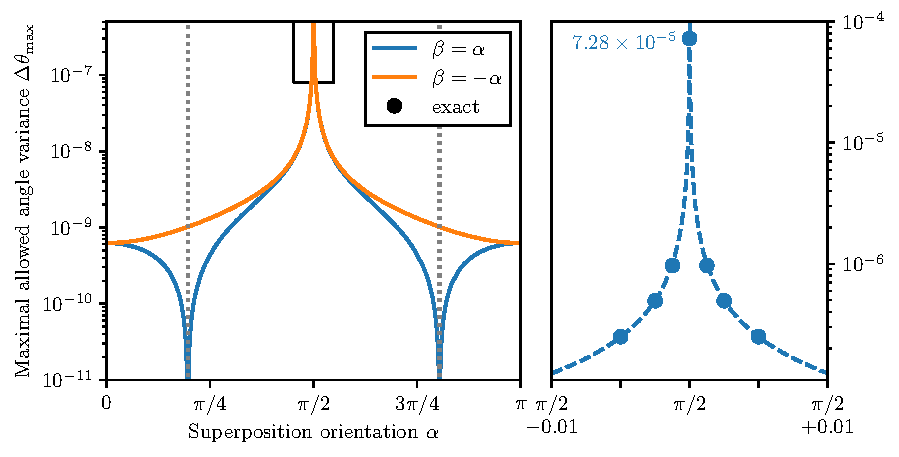
\includegraphics[width=0.95\textwidth]{./../figures/theta-variance/theta-max-orientation-complete.pdf}
  \caption{Maximum possible allowed angular variation $\Delta\theta_\mathrm{max}$ for different orientations. All data-points where calculated at the time of maximum entanglement shown in \cref{fig:4:t-max-orientation}. The \emph{orthogonal configuration} is very stable against angular disturbances. At $\alpha=\beta=\pi/2$, only exact numerical results show a finite value. The singularities on the left figure arise from the fact, that these configurations need infinite time to entangle as already seen in \cref{fig:4:t-max-orientation}.}
  \label{fig:4:theta-max-orientation}
\end{figure}

\begin{figure}[!htbp]
  \centering
  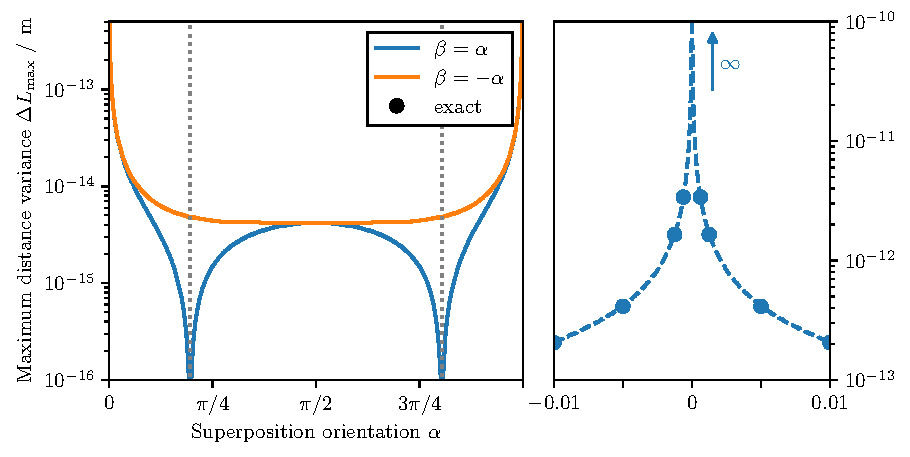
\includegraphics[width=0.95\textwidth]{./../figures/L-variance/L-max-orientation-complete.pdf}
  \caption{Maximum possible allowed distance variation $\Delta L_\mathrm{max}$ for different orientations. This figure is similar to \cref{fig:4:theta-max-orientation}, only for distance variations. On the contrary to angular variations, the \emph{parallel configuration} is infinitely stable against changes in the distance between the shield and the cat-state.}
  \label{fig:4:L-max-orientation}
\end{figure}



\begin{figure}[!htbp]
  \centering
  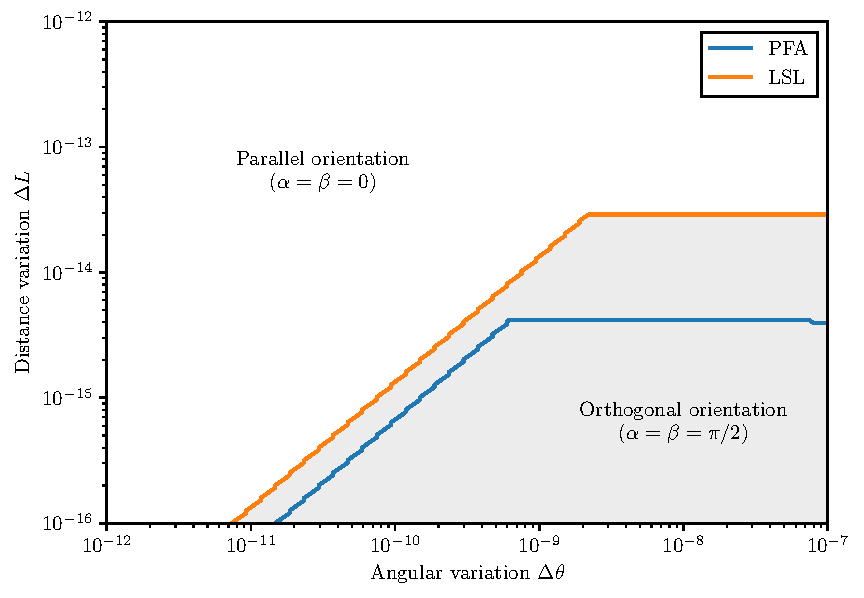
\includegraphics[width=\textwidth]{./../figures/optimize/optimized-orientation.pdf}
  \caption{Optimal orientation for arbitrary variations in the angle $\Delta\theta$ and the distance $\Delta L$. The optimum was calculated for different models of the Casimir-interaction (PFA eq. \eqref{eq:3:PFA-sphere-plate} and LSL eq. \eqref{eq:3:casimir-sphere-plate}).If angular variations dominate, the orthogonal configuration is best, whereas for large distance variations, a parallel orientation is advised.}
  \label{fig:4:optimal-orientation}
\end{figure}